\section{STT-RAM Macro Design Optimization} \label{sec:opt}
In this section we first choose two MTJ specs as our optimization targets. After numerous simulations we the importance of careful write pulse width selection is revealed for optimizing area, read latency/energy, write latency/enery and leakage power of STT-RAM. Then we will focus on the analysis of write energy optimization, which is both device and capacity dependent. Finally we will combine the improved architectural design together with the write pulse width optimization to illustrate a full design explore a STT-RAM chip.

\subsection{Impact of Write Pulse Width}

\begin{figure}[t]
  \centering
  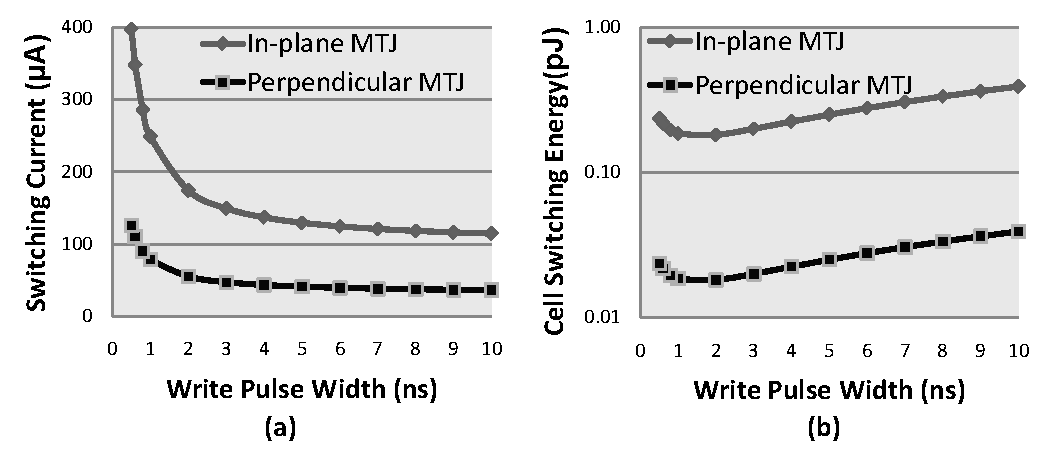
\includegraphics[width=3.5in]{fig/MTJSpec.eps}
  \vspace{-10pt}
  \caption{Representative data curves of in-plane and perpendicular MTJs: (a)Switching current; (b) Cell switching energy.}
  \label{fig:specs}
  \vspace{-5pt}
\end{figure}

As discussed in Section~\ref{subsec:ict}, a wide range of coupled switching current and switching time can be operated for STT-RAM cell. In this work, we will focus on processional switching mode and dynamic reversal mode, particularly, for $0.4ns < \tau < 10ns$. We choose two curves which can represent the typical switching characteristics of in-plane MTJ~\cite{STTRAM:Qualcomm09} and PMTJ~\cite{PMTJ:Toshiba08}. As seen in Figure~\ref{fig:specs}, PMTJ has remarkable advantages over in-plane MTJ in both switching current and switching energy for any given write pulse width assuming the same ratio of damping constant to STT efficiency. The other simulation parameters are listed in~\ref{tb:parameters}. We assume the same TMR and resistance for in-plane MTJ and PMTJ. For PMTJ, realization of matching these parameters of in-plane MTJ needs some device-level efforts as mentioned in Section~\ref{subsec:pmtj}. The minimum write pulse width $\tau_{min\_cell\_energy}$ for each MTJ spec is are extracted from Figure~\ref{fig:specs}(b). Allowed maximum access transistor width is constrained, which has been translated to the operating range of write pulse width.

\begin{table}[t]
\centering
\caption{Simulation Parameters}
\label{tb:parameters}
\vspace{-5pt}
\begin{tabular}{ l | c | c }
\hline \hline
Optimization target & in-plane MTJ & PMJT\\
\hline
Write pulse width operating range & $2ns-10ns$ & $0.4ns-10ns$\\
\hline
$\tau_{min\_cell\_energy}$ & $1.3ns$ & $1.8ns$\\
\hline
TMR & \multicolumn{2}{c}{$120\%$}\\
\hline
LRS Resistance & \multicolumn{2}{c}{$3k\Omega$}\\
\hline
$CTMR_{min}$ & \multicolumn{2}{c}{$60\%$} \\
\hline
Macro Capacity & \multicolumn{2}{c}{$16KB - 4MB$}\\
\hline
Technology Node & \multicolumn{2}{c}{$45ns$}\\
\hline
I/O Width & \multicolumn{2}{c}{$32bits-512bits$}\\
\hline\hline
\end{tabular}
\vspace{-10pt}
\end{table}

NVsim simulation results of 2$MB$ STT-RAM macros with in-plane MTJ and PMTJ separately are compared with SRAM of the same capacity. Different impacts of write pulse width on area, read latency/energy, write latency/energy and leakage power are demonstrated in Figure~\ref{fig:metrics}. In general, decreasing write pulse width will increase area, read latency/energy and leakage power. Especially reducing write pulse with in processional mode will harm these metrics badly. However, the relation between write pulse width and write latency/enery is not monotonous. Separate explanations and result analysis are given,
\begin{itemize}
\item Area: short write pulse induced large switching current requires large access transistor for providing enough driving current, which incur both cell and peripheral circuitry (i.e. wordline driver) area penalty. From Figure~\ref{fig:metrics}(a) we can see that STT-RAM generally has area advantage over SRAM. But reducing write pulse aggressively below $2ns$ will cause STT-RAM with in-plane MTJ to have larger area than SRAM.
\item Read latency: the read timing can be approximately divided into four components: (1) H-tree input/output delay; (2) Decoder + wordline delay; (3) Bitline delay; (4) Sense amplifier delay. (1) is affected because larger area essentially means longer routing distance and interconnection RC delay. Moreover, the increased gate and drain capacitance of larger access transistor will contribute to wordline capacitance and bitline load capacitance, which increase (2) and (3). From Figure~\ref{fig:metrics}(b) we can see that STT-RAM with in-plane MTJ is slightly slower than SRAM mainly because sensing the state of STT-RAM cell takes longer than that of SRAM. However, read operation of STT-RAM with PMTJ can be faster than SRAM for $\tau > 0.8ns$ due to more remarkable area advantage.
\item Read energy: it's affected in the similar way that read latency is affected. From Figure~\ref{fig:metrics}(c) we can see that the read energy of STT-RAM with in-plane MTJ is comparable to that of SRAM while PMTJ improves STT-RAM read energy significantly thus it's better than SRAM.
\item Write latency: the write timing can be approximately divided into four components: (1) H-tree input latency; (2) Decoder + wordline delay; (3) Write pulse width. (1) and (2) both increase as (3) decreases therefore "sweet spots" may exist, which is approved by Figure~\ref{fig:metrics}(d). The write latency of STT-RAM with in-plane MTJ can no longer be improved when $\tau < 3ns$. While the minimum write latency STT-RAM with PMTJ is achieved at $\tau = 0.8ns$ and the latency value is comparable to SRAM.
\item Write energy: it consists of two parts: the energy of cell switching (cell energy) and the energy of the circuitry (peripheral energy) most of which is shared with read operation. When reducing write pulse width from $10ns$ to $\tau_{min\_cell\_energy}$, cell energy decreases while peripheral energy goes up in the same manner with read energy. Later we'll show that the optimal write pulse width $\tau_{min\_energy}$ for minimum write energy is dependent on MTJ spec, STT-RAM capacity and I/O width. We can see from Figure~\ref{fig:metrics}(e) that $\tau_{min\_energy} = 5ns$ for 32-bit 2MB STT-RAM with in-plane MTJ and $\tau_{min\_energy}= 7ns$ for 32-bit 2MB STT-RAM with PMTJ. Moreover, the minimum write energy of STT-RAM with in-plane MTJ is roughly 50\% more than that of SRAM while the energy of STT-RAM with PMTJ is almost half the number of SRAM.
\item Leakage power: leakage power is basically proportional to the sizing of transistor contributing the leakage current. Thus it increases as the area of peripheral circuity increasesl because the leakage power for STT-RAM mainly comes from peripheral circuity. Figure~\ref{fig:metrics}(f) we can tell the remarkable advantage of STT-RAM over SRAM no matter what type of MTJ spec is used.
\end{itemize}


\begin{figure*}[t]
  \centering
  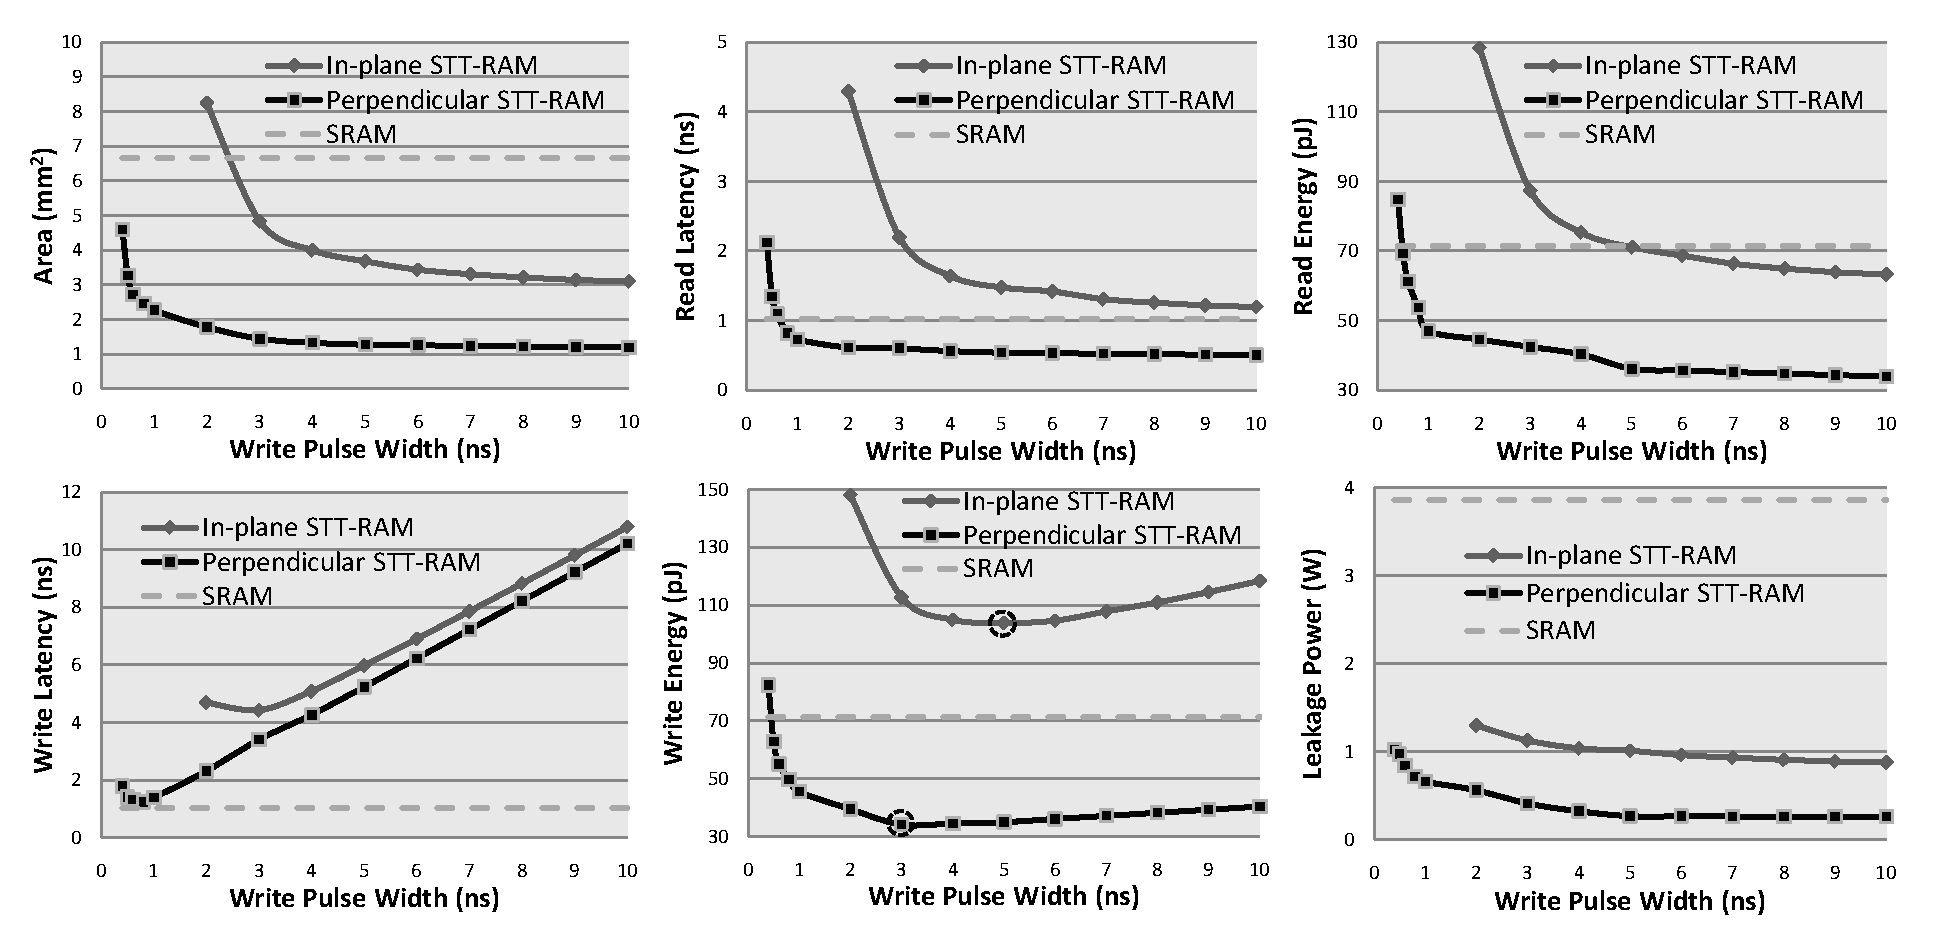
\includegraphics[width=7in]{fig/AllMetrics.eps}
  \caption{Metrics of SRAM and STT-RAM built with in-plane and perpendicular MTJs: (a)Area; (b)Read latency; (c)Read energy; (d)Write latency; (e)Write energy; (f)Leakage power.}
  \label{fig:metrics}
\end{figure*}

\subsection{Write Energy Optimization}
In previous section we note that $\tau_{min\_energy}$ is different for STT-RAM with in-plane MTJ and PMTJ. Thus we did more study on the determining factors and found out $\tau_{min\_energy}$ depends on MTJ spec, STT-RAM capacity and I/O width. From the results shown in Figure~\ref{fig:minenergy}, we observed that: (1) The optimal write pulse width $\tau_{min\_energy}$ for STT-RAM with in-plane MTJ is smaller than that of STT-RAM with PMTJ under the same capacity and I/O Width; (2) $\tau_{min\_energy}$ is a monotonic increasing function of STT-RAM capacity under fixed I/O width (32bits); (3) $\tau_{min\_energy}$ is a monotonic decreasing function of I/O width under fixed capacity (2MB). There are primary two reasons for (1): the baseline $\tau_{min\_cell\_energy}$ of in-plane MTJ than that of PMTJ; proportion of cell energy in PMTJ is much smaller and peripheral energy has more weights on minimizing total energy. (2) is because the proportion of cell energy decreases as capacity increases and peripheral energy begins to decimate at large memory capacity. (3) is due to the similar reason. The conclusions can be viewed as design implications of MTJ device, that is, minimize the cell switching energy at $\tau_{min\_cell\_energy}$ from cell-level may not enough, while it's more important to reduce to cell switching energy at $\tau_{min\_energy}$ for particular capacity and I/O width from system-level point of view.

\begin{figure}[t]
  \centering
  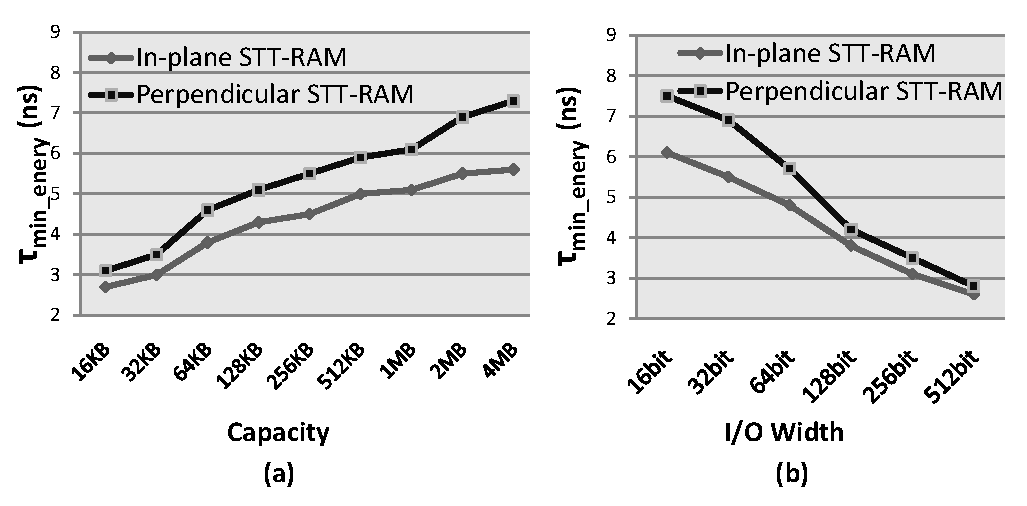
\includegraphics[width=3.5in]{fig/MinEnergy.eps}
  \vspace{-10pt}
  \caption{Dependence of $\tau_{min\_energy}$ on (a) STT-RAM Macro Capacity, and (b) I/O Width}
  \label{fig:minenergy}
  \vspace{-15pt}
\end{figure}

\subsection{Device-Architecture Co-Optimization}

\begin{table*}[t]
%\vspace{-5pt}
\centering
\caption{Device-Architecture Co-Optimization of a 45nm 64MB STT-RAM chip and comparison with DRAM}
\label{tb:bigtable}
%\vspace{-5pt}
\begin{tabular}{| l | c | c | c | c | c | c | c |}
\hline\hline
& Area opt. & Read latency opt. & Write latency opt. & Read energy opt. & Write energy opt. & Leakage opt. &  DRAM \\
\hline
Area ($mm^2$) & \textbf{3.06} & 10.7 & 16.4 & 5.66 & 6.22 & 3.63 & 8.55\\
\hline
Read latency ($ns$) & 21.8 & \textbf{3.70} & 4.92 & 9.12 & 9.57 & 9.91 & 6.24\\
\hline
Write latency ($ns$) & 18.6	& 13.9	& \textbf{4.01}	& 15.9	& 12.3	& 18.1 & 6.24\\
\hline
Read energy ($nJ$) & 0.276	& 0.225	& 0.316	& \textbf{0.105}	& 0.139	& 0.279 & 5.21\\
\hline
Write energy ($nJ$) & 0.293	& 0.322	& 0.309	& 0.193	& \textbf{0.131}	& 0.281 & 4.82\\
\hline
Leakage ($W$) & 1.01	& 3.53	& 4.98	& 1.85	& 1.92	& \textbf{0.78} & 1.83\\
\hline\hline
Write pulse width ($ns$) & 10 & 10 & 2 & 10 & 6 & 10 & - \\
\hline
Inter-array routing & Non-H-tree & H-tree & H-tree & H-tree & H-tree & Non-H-tree & H-tree \\
\hline
Sense amp placement & External & Internal & Internal & Internal & Internal & External & Internal \\
\hline
Sense amp type & Current & Current & Current & Voltage & Voltage & Voltage & Voltage \\
\hline
Interconnect wire & Normal & Repeated & Repeated & Low-swing & Low-swing & Normal & Repeated \\
\hline
Output buffer type & Area opt. & Latency opt. & Latency opt. & Area opt. & Area opt. & Area opt. & Latency opt. \\
\hline\hline
\end{tabular}
%\vspace{-10pt}
\end{table*}

Finally we combine the write pulse width optimization together with other circuit- and architectural- level techniques to design a $64MB$ STT-RAM prototype with 64-bit I/O width under $45nm$ technology node using PMTJ. These optimization choices include: (1) Insert repeaters in interconnection wire to reduce routing delay at the penalty of area and energy; (2) Use partial swing signal for data transfer to reduce energy at the penalty of latency; (3) External sensing scheme with Non-H-Tree routing to reduce chip area; (4) Different buffer design styles for area optimization or latency optimization; (5) Differen sensing schemes for trade-off of area, latency and energy. Table~\ref{tb:bigtable} tabulates the full design spectrum this chip by listing the details of each design corner. Compared the metrics of STT-RAM chip to those of DRAM in the rightmost column, we can see that replacing DRAM by STT-RAM can greatly reduce energy while maintaining performance competitive to DRAM. This is primarily because of elimination of refresh operation due to inherent non-volatility of STT-RAM.

